%!TEX root = ../report.tex
\documentclass[report.tex]{subfiles}
\begin{document}
    \chapter{Methodology}

    How you are planning to test/compare/evaluate your research.
    Criteria used.

        % Dont know where to put DATASET related content
    % One entire section could be my comparative study on multimodal dataset
    \section{Available Datasets}

    % \begin{itemize}
    %     \item The majority of deep multimodal perception approaches rely on supervised learning, and therefore necessitate multimodal datasets with labeled ground truth for training deep neural networks. While several multimodal datasets are available, many of these datasets are collected under clear weather conditions or do not include all sensors, such as cameras, LiDAR, and radar. Unfortunately, the availability of multimodal datasets collected under adverse weather conditions with all three sensors are limited. Table 1 summarizes some of the available multimodal datasets for evaluating the performance of deep multimodal perception techniques in adverse weather conditions. Of these datasets, only the recently released K-Radar \cite{Paek2022Jun} incorporates a high-resolution 4D-radar sensor. In the table, C-R-L-N-F denotes the Camera, Radar, LiDAR, Near-infrared, and Far-infrared sensors, respectively.
    %         \begin{table}[h]
    %             \centering
    %             \caption{List multimodal datasets with adverse weather conditions}
    %             \label{tab:my-table}
    %             \begin{tabular}{|l|l|l|l|}
    %                 \hline
    %                 \textbf{Name}       & \textbf{Sensors} & \textbf{Reference}               & \textbf{Year} \\ \hline
    %                 DENSE               & CRLNF            & \cite{bijelic2020seeing}    & 2020          \\ \hline
    %                 EU Long-term        & CRL              & \cite{yan2020eu}            & 2020          \\ \hline
    %                 nuScenes            & CRL              & \cite{caesar2020nuscenes}   & 2020          \\ \hline
    %                 The Oxford RobotCar & CRL              & \cite{barnes2020oxford}     & 2020          \\ \hline
    %                 RADIATE             & CRL              & \cite{sheeny2021radiate}    & 2021          \\ \hline
    %                 K-Radar             & CRL              & \cite{Paek2022Jun}          & 2022          \\ \hline
    %                 aiMotive            & CRL              & \cite{matuszka2022aimotive} & 2022          \\ \hline
    %                 Boreas              & CRL              & \cite{burnett2022boreas}    & 2022          \\ \hline
    %                 WADS                & CRLNF            & \cite{kurup2022winter}      & 2023          \\ \hline
    %             \end{tabular}
    %         \end{table}

    %         \begin{figure}[h]
    %             \centering
    %             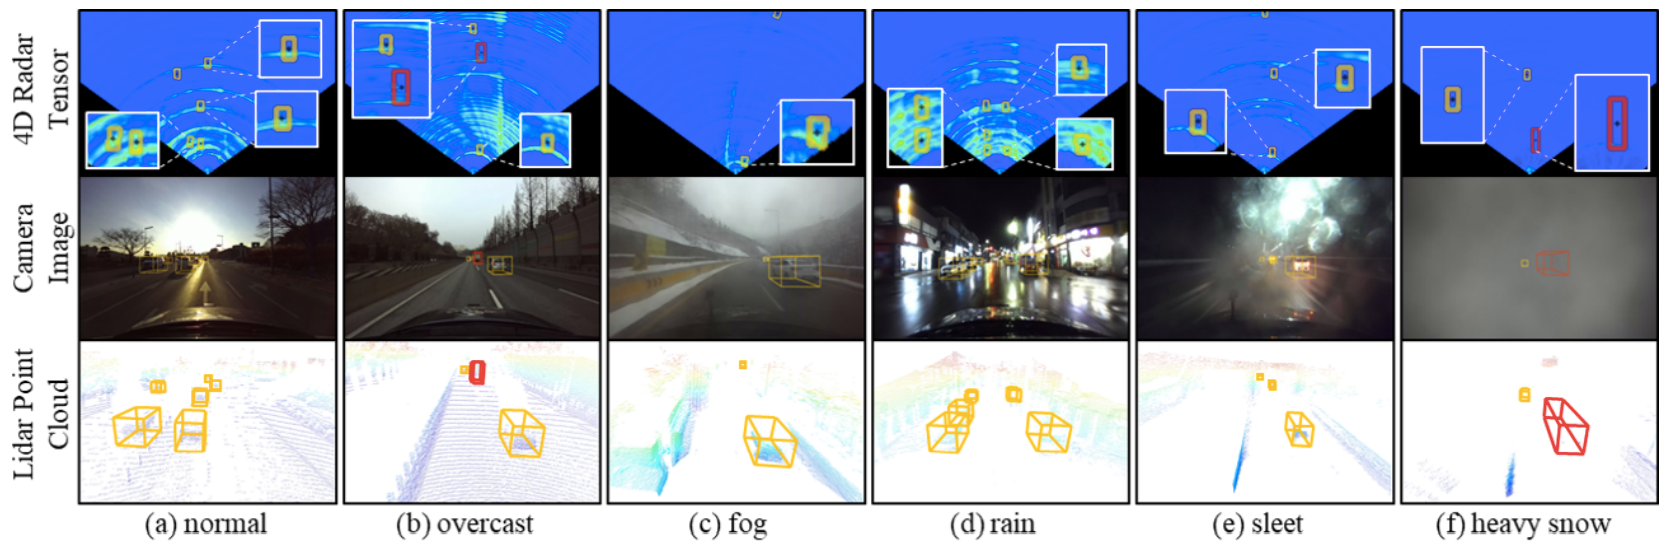
\includegraphics[width=1.0\textwidth]{images/all_sensors_in_adverse_weather.png}
    %             \caption{\centering Samples of K-Radar datasets for various weather conditions \cite{Paek2022Jun}}
    %             \label{fig:all_sensors_in_adverse_weather}
    %         \end{figure}
    %     \end{itemize}


    The majority of deep multimodal perception approaches rely on supervised learning, which necessitates the use of high-quality, large-scale multimodal datasets with labeled ground truth for training deep neural networks. Several multimodal datasets, such as KITTI \cite{geiger2012we}, ApolloScape \cite{huang2019apolloscape}, and Waymo \cite{sun2020scalability}, are prevalent in the domain of LiDAR-camera fusion. However, a significant number of these datasets are collected under clear weather conditions or lack a comprehensive array of sensors, including cameras, LiDAR, and Radar. A notable limitation is the scarcity of multimodal datasets that are collected under adverse weather conditions and incorporate at least all three of these essential sensors. Table \ref{datasets} summarizes some of the available multimodal datasets\footnote{For all the datasets, formal registration form is required to fill to access the dataset} for evaluating the performance of deep multimodal perception techniques in adverse weather conditions. Note that highlighted datasets are used for the project. The dataset are sorted in ascending order with respect to year.
    
    TODO: add histogram of object classes for DENSE and nuScenes datasets

    \begin{table}[!ht]
        \centering
        \caption{Multimodal Adverse Weather Conditions Datasets. Sensors†: C-R-L-N-F denote Camera, Radar, LiDAR, Near-infrared, and Far-infrared sensors, respectively. Weather Conditions‡: F-SN-R-O-SL-N denote Fog, Snow, Rain, Overcast, Sleet, and Night conditions, respectively.}
        \begin{tabular}{|l|l|l|l|l|l|l|}
        \hline
            \textbf{Name} & \textbf{Sensors†} & \textbf{Weather Cond.‡} & \textbf{Size (GB)} & \textbf{Year} & \textbf{Citation Cnt.} & \textbf{Reference} \\ \hline
            \textbf{DENSE} & \textbf{CRLNF} & \textbf{F, SN, R, N} & \textbf{582} & \textbf{2020} & \textbf{269} & \textbf{\cite{bijelic2020seeing}} \\ \hline
            \textbf{nuScenes} & \textbf{CRL} & \textbf{R, N} & \textbf{400} & \textbf{2020} & \textbf{3459} & \textbf{\cite{caesar2020nuscenes}} \\ \hline
            The Oxford RobotCar & CRL & R, SN, F & 4700 & 2020 & 317 & \cite{barnes2020oxford} \\ \hline
            EU Long-term & CRL & SN, R, O, N & NA & 2020 & 72 & \cite{yan2020eu} \\ \hline
            RADIATE & CRL & F, SN, R, O, SL, N & NA & 2021 & 132 & \cite{sheeny2021radiate} \\ \hline
            K-Radar & CRL & F, R, SN & 13000 & 2022 & 15 & \cite{Paek2022Jun} \\ \hline
            Boreas & CRL & SN, R, O, N & 4400 & 2022 & 38 & \cite{burnett2022boreas} \\ \hline
            aiMotive & CRL & R, O, N & 85 & 2023 & 3 & \cite{matuszka2022aimotive} \\ \hline
        \end{tabular}
        \label{datasets}
    \end{table}


    The datasets for the project are selected based on the following criteria:
    - Available Sensors, at least it should have camera, radar, and lidar
    - Adverse weather conditions,
    - Dataset documentation and accessibility,
    - Usage by publicly available methods (so that comparison is possible)
    - Perception Task, eg. Object Detection
    - Radar datatype, the data should be available in point cloud format
    - Time-synchronized and calibrated data

    After considering above criteria, the following datasets are selected (also highlighted in the table): 
    - DENSE
    - nuScenes

    \subsection{DENSE dataset \cite{bijelic2020seeing}}

    TODO: paraphrase
    The Dense dataset \cite{bijelic2020seeing} focused on evaluating multi-modal fusion algorithms under adverse weather. In addition to LiDAR and a stereo camera, it is also equipped with several all-weather sensors, including one frontal long-range radar, one gated camera working on the NIR band, one FIR camera, and one weather station sensor. The data are captured in various natural weather conditions, including rain, snow, light fog, and heavy fog, as well as in a controlled lab environment in a fog chamber. However, the dataset only provides sparse radar targets with limited FoV and poor resolution. The dataset is recorded in urban city, suburban, highway, and tunnel areas. It coveres several weather conditions like light fog, dense fog, rain, snow, and night. The dataset is used by several multimodal sensor fusion publications for object detection. Table \ref{tab:dataset_comparison} higlihts the sensor setup and dataset statistics for each dataset. Geographical coverage of the data collection campaign covering two months and 10,000 km in Germany,
    Sweden, Denmark, and Finland. 
    % Scenarios: U, S, H, and T stand for urban (city), suburban, highway, tunnel
    % Radar datatype: pointcloud

    \begin{table}[h!]
        \centering
        \begin{tabular}{|l|c|c|}
          \hline
          \textbf{Dataset} & \textbf{NuScenes \cite{caesar2020nuscenes}} & \textbf{DENSE \cite{bijelic2020seeing}} \\
          \hline
          Sensor Setup & 6 & 2 \\
          RGB Cameras & 6 & 2 \\
          RGB Resolution & 1600x900 & 1920x1024 \\
          Lidar Sensors & 1 & 2 \\
          Lidar Resolution & 32 & 64 \\
          Radar Sensor & 4 & 1 \\
          Gated Camera & x & 1 \\
          FIR Camera & x & 1 \\
          Frame Rate & 1 Hz/10 Hz & 10 Hz \\
          \hline
          \textbf{Dataset Statistics} &  &  \\
          \hline
          Labeled Frames & 40K & 13.5K \\
          Labels & 1.4M & 100K \\
          Scene Tags & \checkmark & \checkmark \\
          Night Time & \checkmark & \checkmark \\
          Light Weather & \checkmark & \checkmark \\
          Heavy Weather & x & \checkmark \\
          Fog Chamber & x & x \\
          \hline
        \end{tabular}
        \caption{Comparison of Dataset Features}
        \label{tab:dataset_comparison}
      \end{table}
      

        \begin{figure}[h]
                \centering
                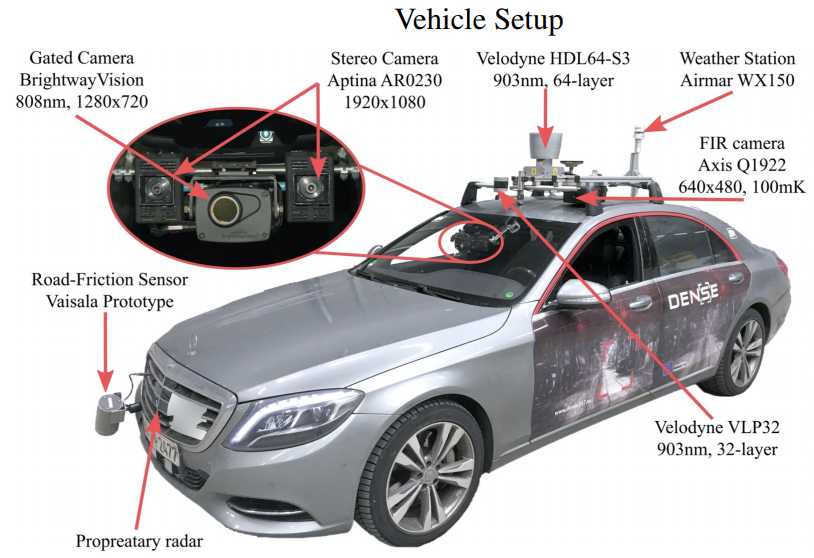
\includegraphics[width=0.9\textwidth]{images/datasets/dense/test_vehicle_setup.png}
                \caption{Test Vehicle Setup \cite{bijelic2020seeing}}
                \label{fig:dense_test_vehicle_setup}
        \end{figure}

        \begin{figure}[h]
                \centering
                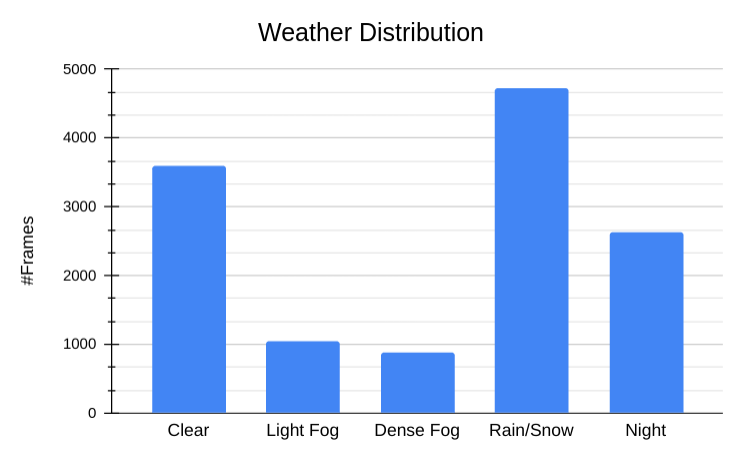
\includegraphics[width=0.9\textwidth]{images/datasets/dense/distribution_of_weather_conditions.png}
                \caption{Distribution of Weather Conditions \cite{bijelic2020seeing}}
                \label{fig:dense_distribution_of_weather_conditions}
        \end{figure}


    \subsection{nuScenes dataset \cite{caesar2020nuscenes}}

    NuScenes \cite{caesar2020nuscenes} is the most popular dataset for its large-scale and diverse scenarios. The capturing vehicle is equipped with a 32-beam LiDAR, 6 cameras, 5 long-range multi-mode radars, and a GPS/IMU system. It provides 3D annotations of 23 classes of road users in 1000 scenes, with a total of 1.3 million frames. Although, the radar used in nuScenes has a sparse data, but it is good dataset to start with and also well documented.
    Scenarios: U, S, and H stand for urban (city), suburban, highway
    Radar datatype: pointtcloud

    
    % Table in descending order w.r.t. year
    % \begin{table}[!ht]
    %     \centering
    %     \caption{Multimodal Adverse Weather Conditions Datasets}
    %     \begin{tabular}{|l|l|l|l|l|l|l|}
    %     \hline
    %         \textbf{Name} & \textbf{Sensors *} & \textbf{Link} & \textbf{Year} & \textbf{Size (GB)} & \textbf{Weather Cond.**} & \textbf{Citation} \\ \hline
    %         aiMotive & CRL & Link & 2023 & 85 & R, O, N & 3 \\ \hline
    %         K-Radar & CRL & Link & 2022 & 13000 & F, R, SN & 15 \\ \hline
    %         Boreas & CRL & Link & 2022 & 4400 & SN, R, O, N & 38 \\ \hline
    %         RADIATE & CRL & Link & 2021 & ~ & F, SN, R, O, SL, N & 132 \\ \hline
    %         \textbf{DENSE} & \textbf{CRLNF} & \textbf{Link} & \textbf{2020} & \textbf{582} & \textbf{F, SN, R, N} & \textbf{269} \\ \hline
    %         \textbf{nuScenes} & \textbf{CRL} & \textbf{Link} & \textbf{2020} & \textbf{400} & \textbf{R, N} & \textbf{3459} \\ \hline
    %         The Oxford RobotCar & CRL & Link & 2020 & 4700 & R, SN, F & 317 \\ \hline
    %         EU Long-term & CRL & Link & 2020 & ~ & SN, R, O, N & 72 \\ \hline
    %     \end{tabular}
    %     \label{datasets}
    % \end{table}

    % Table in ascending order w.r.t. year
    % \begin{table}[!ht]
    %     \centering
    %     \caption{Multimodal Adverse Weather Conditions Datasets}
    %     \begin{tabular}{|l|l|l|l|l|l|l|}
    %     \hline
    %         \textbf{Name} & \textbf{Sensors *} & \textbf{Weather Cond.**} & \textbf{Size (GB)} & \textbf{Year} & \textbf{Citation Cnt.} & \textbf{Reference} \\ \hline
    %         \textbf{DENSE} & \textbf{CRLNF} & \textbf{F, SN, R, N} & \textbf{582} & \textbf{2020} & \textbf{269} & \textbf{\cite{bijelic2020seeing}} \\ \hline
    %         \textbf{nuScenes} & \textbf{CRL} & \textbf{R, N} & \textbf{400} & \textbf{2020} & \textbf{3459} & \textbf{\cite{caesar2020nuscenes}} \\ \hline
    %         The Oxford RobotCar & CRL & R, SN, F & 4700 & 2020 & 317 & \cite{barnes2020oxford} \\ \hline
    %         EU Long-term & CRL & SN, R, O, N & ~ & 2020 & 72 & \cite{yan2020eu} \\ \hline
    %         RADIATE & CRL & F, SN, R, O, SL, N & ~ & 2021 & 132 & \cite{sheeny2021radiate} \\ \hline
    %         K-Radar & CRL & F, R, SN & 13000 & 2022 & 15 & \cite{Paek2022Jun} \\ \hline
    %         Boreas & CRL & SN, R, O, N & 4400 & 2022 & 38 & \cite{burnett2022boreas} \\ \hline
    %         aiMotive & CRL & R, O, N & 85 & 2023 & 3 & \cite{matuszka2022aimotive} \\ \hline
    %     \end{tabular}
    %     \label{datasets}
    % \end{table}


    
    



    \section{Setup}

    \section{Experimental Design}

    \section{Evaluation Metrics}

    

\end{document}
